\documentclass[12pt, a4paper]{article}

\usepackage[T2A]{fontenc}
\usepackage[utf8]{inputenc}
\usepackage[english, russian]{babel}
\usepackage{amssymb}
\usepackage{amsfonts}
\usepackage{amsmath}
\usepackage{mathtext}

\usepackage{comment}
\usepackage{geometry}
\geometry{left=1cm, right=1cm, top=2cm, bottom=2cm}

\usepackage{graphicx}
\usepackage{tikz}

\usepackage{wrapfig}
\usepackage{fancybox,fancyhdr}
\sloppy

\setlength{\headheight}{28pt}

\newcommand{\head}[4]
{
	\fancyhf{}
	\pagestyle{fancy}
	\chead{#3, #4}

	\begin{center}
	\begin{large}
	#1 \\
	\textit{#2} \\
	\end{large}
	\end{center}

}

\begin{document}

\head{VIII Республиканская студенческая предметная олимпиада по направлению \\ <<Математика>>}{01 апреля 2016}{Казахстанский филиал МГУ имени М. В. Ломоносова}{г. Астана}

\begin{enumerate}

\item (Васильев А.Н.)

Заметим, что справедливо разложение $$x^2-y^2+2x+2y = (x+y)(x-y+2).$$ Поэтому натуральное число представимо в этом виде тогда, и только тогда, когда раскладывается на произведение двух множителей одной четности. Ясно, что это все числа, которые дают остаток отличный от 2 при делении на 4.

Пример для нечетного $n$: $x = \frac{n-1}{2}$, $y = \frac{3-n}{2}$.

Пример для $n$, кратного 4: $x = y = \frac{n}{4}$.
 
\item (Васильев А.Н.) 

а) Легко понять, что функция кусочно--постоянная. Причем количество промежутков постоянства конечно и равно 10. Значит, функция интегрируема по Риману. 
\\
б) Найдем промежуток, на котором первая цифра числа $2^x$ равна $k$:
$$1 + \frac{k}{10} \le 2^x < 1 + \frac{k+1}{10},$$
$$\log_2 \left( 1 + \frac{k}{10} \right) \le x < \log_2 \left( 1 + \frac{k+1}{10} \right).$$

Тогда наш интеграл можно записать в виде суммы:
\begin{multline*}
\int\limits_{0}^{1} \alpha(x) dx = \\
= \sum_{k=0}^{9} k \left( \log_2 \left( 1 + \frac{k+1}{10} \right) - \log_2 \left( 1 + \frac{k}{10} \right) \right) = \\
= \sum_{k=0}^{9} k \left( \log_2 (k+11) - \log_2 (k+10) \right) = \\
= \sum_{k=0}^{9} k \log_2 (k+11) -  \sum_{k=0}^{8} (k + 1) \log_2 (k + 11) = \\
= 9 \log_2 20 - \sum_{k=0}^{8} \log_2 (k + 11) = \log_2 \frac{20^9}{11 \cdot 12 \cdot \ldots \cdot 19}
\end{multline*}

Требуется доказать, что
$$2^7 < \left( \frac{20^9}{11 \cdot 12 \cdot \dots \cdot 19} \right)^2 < 2^9.$$

Докажем левую часть неравенства. Заметим, что по неравенству Коши 
$$(10+k) * (20-k) < \left( \frac{10+k+20-k}{2} \right)^2 = 15^2.$$
Отсюда получается оценка слева:
$$\left( \frac{20^9}{11 \cdot 12 \cdot \ldots \cdot 19} \right)^2 > \left( \frac{20^9}{15^9} \right)^2 = \frac{2^{36}}{3^{18}}.$$

Остается доказать, что $2^{29} > 3^{18}$. Заметим, что $2^8>3^5$ и $2^5>3^3$. Перемножив три раза первое неравенство и один раз второе, получим требуемое.

Докажем правую часть неравенства. Заметим, что верно следующее неравенство:
$$(10+k) (20-k) = 200 + k (10 - k) > 200.$$

Значит, оценку справа можно получить так:
$$\left( \frac{20^9}{11 \cdot 12 \cdot \ldots \cdot 19} \right)^2 < \left( \frac{400^4 \cdot 20}{200^4 \cdot 15} \right)^2 = 2^8 \left( \frac{4}{3} \right)^2 < 2^9.$$


\item (Фольклор) Первое решение (<<наивное>>). Можно доказать более общее утверждение:

\textit{В любом конечном поле $F \ne Z_2$ сумма всех элементов равна нулю.}

Пусть $F$ --- конечное поле и $a_1$, $a_2$, ..., $a_n$ --- все его элементы. Если $F \ne Z_2$, то существует элемент $a$, отличный от нуля и единицы. Тогда $a a_1$, $a a_2$, ..., $a a_n$ попарно различны, следовательно
$$F = \{ a_1, ..., a_n \} = \{ a a_1, ..., a a_n \} .$$
Отсюда $S = \sum_{i=1}^{n} a_i = \sum_{i=1}^n a a_i = a S$, откуда следует, что $S = 0$.

Второе решение(существенно использующее структуру конечного поля). Утверждение из предыдущего решения можно доказать и по-другому. Ненулевые элементы поля образуют группу по умножению, а порядок элемента группы делит порядок группы (по теореме  Лагранжа). Следовательно, любой элемент поля $F$ является корнем многочлена $x^n - x = 0$, где $n$ --- количество элементов поля. С другой стороны, по другой теореме Лагранжа, у этого многочлена не более $n$ корней. Иными словами, указанный многочлен имеет своими корнями все элементы поля. Применяя теорему Виета, получаем требуемое. 

Третье решение (еще одно). У каждого ненулевого элемента $x$ есть обратный $x^{-1}$, причем $x \ne x^{-1}$ при $x \ne \pm 1$. Следовательно, все ненулевые элементы, кроме $\pm 1$, разбиваются на пары с произведением 1. Поэтому произведение всех элементов поля равно $-1$. Из условия задачи следует, что $-1 \ne 1$. Следовательно, характеристика поля отлична от 2. Тогда любой ненулевой элемент отличается от своего противоположного, то есть все ненулевые элементы разбиваются на пары с нулевой суммой. Что означает, что сумма всех ненулевых элементов поля равна нулю. Добавление нуля сумму не изменяет. Утверждение доказано.    

\item  (Баев А.Ж.) 

Факт 1 (оптическое свойство эллипса): луч, направленный из одного фокуса после отражения от внутренней стороны эллипса проходит через другой фокус. То есть $\angle(F_1M, SM) = \angle(SM, F_2M)$, где $\angle(l_1, l_2)$ обозначает ориентированный угол между прямыми. Как следствие, получаем, что $\angle F_1MS + \angle F_2MS = \pi$. По условию, $\angle F_2MS = \angle DMS$. Откуда получаем, что $F_1$, $M$, $D$ лежат на одной прямой. Аналогично, $F_2$, $N$, $E$ лежат на одной прямой.

Факт 2 (определение эллипса). Сумма расстояний от фокусов до точек на эллипсе постоянна. Как следствие $F_1M + MF_2 = F_1N + NF_2$. Так как треугольники $F_2MS$ и $DMS$ симметричны относительно прямой $MS$, то и треугольники $F_1MF_2$ и $AMD$ тоже симметричны и, соответственно, равны. Аналогично, симметричны и равны треугольники $F_1NF_2$ и $BNE$.

\begin{center}
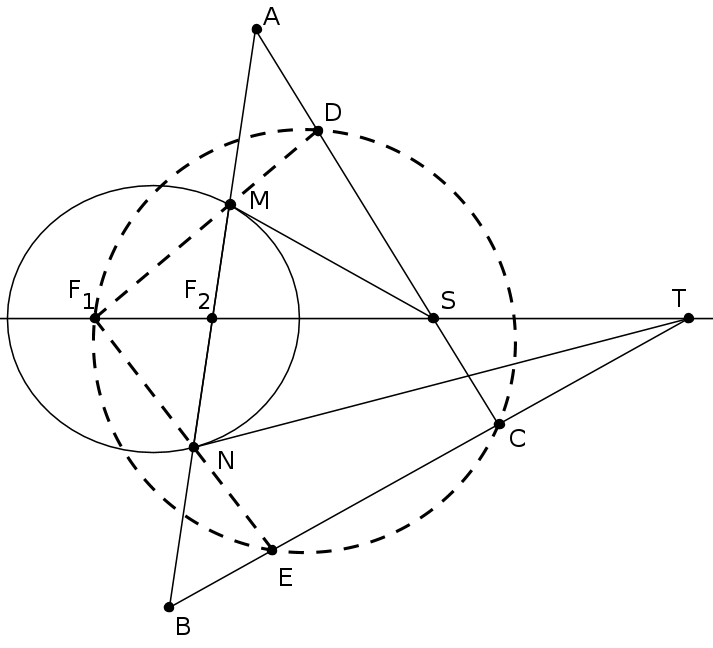
\includegraphics[width=8cm]{pictures/2016-republic}
\end{center}

а) 
$$AF_2 = AM + MF_2 = F_1M + MF_2 =$$
$$= F_1N + NF_2 = BN + NF_2 = BF_2.$$ 
Значит, $CF_2$ --- медиана треугольника $ABC$.

б) Четырехугольник $F_1DCE$ вписан в окружность, так как $\angle F_1DC + \angle F_1EC = \angle MF_2S + \angle NF_2S = \pi$. Так как в этом четырехугольнике две смежные стороны равны ($F_1D = F_1E$), то $CF_1$ --- биссектриса треугольника $ABC$.

\item (Клячко А.А.)

1) Рассмотрим случай четного $n$. Тогда каждый из игроков полностью контролирует $\frac{n}{2}$ столбцов (при этом не имеет значения, кто делает первый ход). Ясно, что Максималист может сделать свои столбцы линейно независимыми и обеспечить ранг матрицы минимум $\frac{n}{2}$. Также ясно, что Минималист может сделать все свои столбцы нулевыми, ограничив ранг матрицы $\frac{n}{2}$.

Ответ для четного $n$: $\frac{n}{2}$.

2) Пусть $n$ нечетно. Тогда, если мы раскрасим клетки таблицы в черный и белый цвета в шахматном порядке, каждый из игроков будет контролировать клетки одного цвета. 

а) Пусть Максималист делает первый ход. Тогда он сможет сделать ранг матрицы максимальным, то есть равным $n$. Опишем его стратегию. Она состоит в том, что, заполняя очередную диагональную клетку, он следит за тем, чтобы соответствующий главный (угловой) минор был отличен от нуля. Это всегда можно обеспечить, поскольку этот минор разлагается по своей последней строке, а алгебраическое дополнение последнего элемента не равно нулю. 
Ответ для нечетного $n$, когда Максималист делает первый ход: $n$. 

б) Пусть Минималист делает первый ход. Тогда он сможет обеспечить равенство нулю определителя всей матрицы: заполняя очередную диагональную клетку (кроме последней), он следит за тем, чтобы соответствующий угловой минор был отличен от нуля, а в конце обнуляет определитель всей матрицы. Значит, он сможет гарантировать ранг меньше $n$. С другой стороны, Максималист сможет обеспечить, чтобы минор, полученный вычеркиванием последней строки и первого столбца, был отличен от нуля (аналогично пункту 2 а)). Тем самым, ранг матрицы будет равен по крайней мере $n-1$. 

Ответ для нечетного $n$, когда Минималист делает первый ход: $n-1$. 
 
\item (Баев А.Ж.)

1 шаг. Подставим в соотношение $x = \frac{t}{t-1}$, где $t > 1$. Получим
$$f'\left(\frac{t}{t-1}\right) = f(t) + f\left( \frac{t}{t-1} \right) .$$

Получим свойство:
$$f' \left(\frac{t}{t-1} \right) = f'(t).$$

2 шаг. Продифференцируем исходное соотношение по $x$.
$$ f''(x) = - \frac{1}{(x-1)^2} f' \left( \frac{x}{x-1} \right) + f'(x) .$$

После замены из свойства, получаем:
$$ \frac{f''(x)}{f'(x)} = 1 - \frac{1}{(x-1)^2} .$$

Уравнение интегрируется по частям:
$$ f'(x) = C e^{x + \frac{1}{x-1}}.$$

Добавим условие на бесконечности и найдем $C = 1$:
$$ f'(x) = 2 e^{x + \frac{1}{x-1}}.$$

3 шаг. Заметим, что если в исходное дифференциальное уравнение мы подставим $x = 2$, то получим $f(2) = \frac{1}{2} f'(2)$. Значит:
$$ f(2) = e^3.$$

Осталось доказать, что $e^3 < 20.16$. Заметим, что для проверки этого неравенства грубых оценок типа $e<3$ или $e<2.8$ недостаточно, требуется более точная: $e<2.72$.

\end{enumerate}

\end{document} 
